\documentclass[a4paper, pagesize=pdftex, pdftex, twoside, headsepline, index=totoc,toc=listof, fontsize=10pt, cleardoublepage=empty, headinclude, DIV=13, BCOR=13mm]{scrartcl}

\usepackage[ngerman]{babel}
\usepackage{scrtime} % Bestandteil von KOMA-Skript, ermoeglicht Zugriff auf Uhrzeit des Kompilierens 
\usepackage{scrpage2} % ermöglicht Bearbeiten von Kopf- und Fusszeilen (wie fancyhdr, nur optimiert auf KOMA-Skript, leich andere Syntax)
\usepackage[utf8]{inputenc} % Gibt an in welcher Textcodierung der Code verstandne werden soll
\usepackage{etex} % sehr technisch, ermöglicht LaTeX mehr Speicher zu belegen
\usepackage[T1]{fontenc} % auch sehr technisch; ist wichtig, um die Schriftarten richtig zu behandeln
\usepackage{textcomp} %verhindert ein paar Fehler bei den Fonts
\usepackage{amsmath} % Packet der American Mathematical Society, das viele Mathematik-Umgebungen und -Befehle definiert
\usepackage{amssymb} %zusätzliche Symbole
\usepackage{latexsym} % nochmal zusätzliche Symbole
\usepackage{stmaryrd} % nochmal mehr zusätzliche Symbole, u.a. Blitz für Widerspruchsbeweise ;)
\usepackage{nicefrac} % schräge Brüche, benutzte ich für Quotienvektorräume
\usepackage{paralist} % redefiniert alle Listenbefehle, sodass diese einen optionalen Parameter haben, der die Nummerierung angibt
\usepackage{dsfont} % Schriftart für N,Z,Q,R die ich momentan benutze (mittels \mathds{R} z.B)
\usepackage[pdftex]{graphicx} % Packet, dass das Einbinden von Grafiken aus Dateien ermöglicht
\usepackage{makeidx}% ermöglicht das automatische Anlegen eines Index 
\usepackage{extarrows}
\usepackage{bbold} %indikatorfkt
\usepackage{mathtools}

\flushbottom
\usepackage[normalem]{ulem}
\setlength{\ULdepth}{1.8pt}

%--Indexverarbeitung
\newcommand{\bet}[1]{\uline{\textbf{#1}}} %Betonung von Text
\newcommand{\Index}[1]{\uline{\textbf{#1}}\index{#1}} % Befehl, der gleichzeitg das Argument hervorhebt und in den Index mitaufnimmt
\makeindex % startet das automatische Sammeln der Index-Einträge
% Ein kleiner Text am Anfang des Index
\setindexpreamble{{\noindent \itshape Die \emph{Seitenzahlen} sind mit Hyperlinks zu den entsprechenden Seiten versehen, also anklickbar!} \par \bigskip}
\renewcommand{\indexpagestyle}{scrheadings} % Seitenstil für den Index festlegen

%--Farbdefinitionen
\usepackage[usenames, table, x11names]{xcolor} %usenames und x11names, aktivieren viele Farben; siehe Dokumentation von xcolor
% Es lassen sich natürlich auch eigene Farben definieren (hier nur Graustufen)
\definecolor{dark_gray}{gray}{0.45}
\definecolor{light_gray}{gray}{0.7}

%--Zum Zeichnen (ich habe es jetzt mal mit aufgenommen, aber es ist eigentlich nochmal ein ganz anderes Thema, sodass ich da jetzt nicht viel zu sagen werde)
\usepackage{tikz} % TikZ steht übrigens für "TikZ ist kein Zeichenprogramm", ein rekursives Akronym ...
\tikzset{>=latex}
\usetikzlibrary{shapes,arrows}
\usetikzlibrary{calc}
\usetikzlibrary{decorations.pathreplacing}
% Hiermit kann man ganz leicht kommutative Diagramme zeichnen (deswegen auch "cd")
\usepackage{tikz-cd}

%--Marginnote, ermöglicht es kleine Notizen an neben den eigentlichen Textkörper zu setzten
\usepackage{marginnote}
\renewcommand*{\marginfont}{\color{Honeydew4} \footnotesize }

%--Schriftarten
\usepackage{lmodern} % neuere Version der Standard-LaTeX-Schriftarten
\renewcommand{\familydefault}{\sfdefault} %Standardschriftart auf die serifenlose Schriftart setzen

%--Hyperref; aktiviert Hyperlinks in der erzeugten PDF-Datei und definiert deren Aussehen
\usepackage[colorlinks, pdfpagelabels, pdfstartview=FitH, bookmarksopen=true, bookmarksnumbered=true,linkcolor=black,urlcolor=SkyBlue2, plainpages=false, hypertexnames=false, citecolor=black, hypertexnames=true]{hyperref}

%--Römische Zahlen
\newcommand{\RM}[1]{\MakeUppercase{\romannumeral #1{}}}



%-- Definitionen von weiteren Mathe-Befehlen, die dann das "richtige" Aussehen haben. Hier sind der Phantasie keine Grenzen gesetzt
\DeclareMathOperator{\id}{id} %identische Abbildung
\DeclareMathOperator{\End}{End} %Endomorphismen
\DeclareMathOperator{\rg}{rg} %Rang
\DeclareMathOperator{\diam}{diam} %Durchmesser
\DeclareMathOperator{\dist}{dist} %Distanz
\DeclareMathOperator{\grad}{grad} %Gradient
\DeclareMathOperator{\rot}{rot} %Rotation
\DeclareMathOperator{\hess}{Hess} %Hesse-Matrix


%--Skalarprodukt (cooler Befehl, den ich im Internet gefunden habe; benutzt TeX-Befehle)
\makeatletter
\newcommand{\sprod}[2]{\ensuremath{%
  \setbox0=\hbox{\ensuremath{#2}}
  \dimen@\ht0
  \advance\dimen@ by \dp0
  \left\langle \left.#1 \,\rule[-\dp0]{0pt}{\dimen@}\right|#2\right\rangle}}
\makeatother

%--Norm (auch aus dem Internet, wird auch auf der Beispielseite verwandt)
\newcommand{\norm}[2][\relax]{
\ifx#1\relax \ensuremath{\left\Vert#2\right\Vert}
\else \ensuremath{\left\Vert#2\right\Vert_{#1}}
\fi}


%--selbstgeschriebenen Befehle
%--Betrag
\newcommand{\abs}[1]{\ensuremath{\left\vert#1\right\vert}}

%--Umklammern mit passender Größe der Klammern
\newcommand{\enbrace}[1]{\ensuremath{\left( #1\right)}}

%--Mengen
\newcommand{\penbrace}[1]{\ensuremath{\left\{#1\right\}}}

%--Differential
\newcommand{\diff}[2]{\ensuremath{\frac{\partial #1}{\partial #2} }}

\newcommand{\zz}{$\mathrm{Z\kern-.3em\raise-0.5ex\hbox{Z}}$} % zu zeigen ZZ aus dem inet
\setlength{\parindent}{0pt}%absatz nicht einrücken



%--Konfiguration von scrheadings (hierzu findet man auch massig zusätzliche Infos im scrguide)
\setheadsepline{1pt}[\color{light_gray}] 
\pagestyle{scrheadings} %definiert welcher Seitenstil im Dokument normalerweise verwendet werden soll
\clearscrheadfoot % erstmal alles, was eventuell in Kopf- und Fusszeile steht, löschen

% ohead steth für "outer Head", auf einer linken Seite als für den linken Kopf, auf einer rechten für den rechten (es wird ja ein doppelseitiges Layout verwandt)
% durch den hfill-Befehl wird die allesdings untergraben, was aber von mir beabsichtig ist
\ohead{\footnotesize \sffamily \color{light_gray} 
\includegraphics[height=0.5 cm, keepaspectratio]{Bilder/Logo_WWU_Muenster_light_gray.jpg}
	
\includegraphics[height=0.4cm, keepaspectratio]{Bilder/fb10logo.jpg}
	Tobias Wedemeier -- Finanzmathematik
	\hfill { \tiny \sffamily \color{light_gray} Stand: \today \; \thistime[:]}}

% durch den optionalen Parameter (eckige Klammern) wird auch der plain-Pagestyle bearbeitet, damit auch auf leeren Seiten die Seitenzahl steht
\ofoot[{ \color{dark_gray} \LARGE \sffamily \thepage}]{{ \color{dark_gray} \LARGE \sffamily \thepage}} 

% hier wird die aktuelle section in den "inner foot" gesetzt
\automark{section}
\ifoot{ \color{dark_gray} \small \leftmark}

%--Metadaten, die durch den \maketitle gesetzt werden
\author{Tobias Wedemeier}
\titlehead{
\includegraphics[width=7cm, keepaspectratio]{Bilder/Logo_WWU_Muenster_light_gray.jpg} \hfill 
\includegraphics[width=6cm, keepaspectratio]{Bilder/fb10logo.jpg}}
\title{Finanzmathematik}
\subtitle{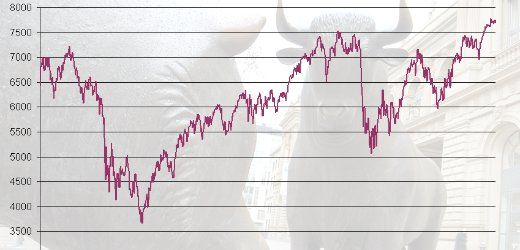
\includegraphics[width=9cm]{Bilder/boerse.jpg}}
\publishers{gelesen von \\ PD Dr. Paulsen}





\begin{document}
\maketitle
\thispagestyle{empty}
\newpage

\thispagestyle{empty}
\vspace*{\fill}
\begin{center}
	Hierbei handelt es sich um eine Mitschrift der Vorlesung von \textbf{PD Dr. Paulsen}, WWU Münster, aus der Vorlesung \textbf{Finanzmathematik} im Wintersemester 2014/15. Dies ist kein Skript der Vorlesung und keine eigene Arbeit des Autors.\\
	\vspace{2cm}
	Für Fehler in der Mitschrift wird keine Haftung übernommen. Hinweise auf Fehler sind gerne gesehen, hierfür kann man mich in der Uni ansprechen oder alternativ eine e-Mail an: \textit{tobias.wedemeier@gmx.de}\\
	Auch ist eine Mitarbeit über Github möglich.\\
	\vspace{2cm}
	Wenn Teile aus der Vorlesung selber fehlen, können diese gerne an meine e-Mail versandt werden. Ich werde diese dann einarbeiten.
\end{center}
\vspace*{\fill}
\newpage

\pagenumbering{Roman}

\tableofcontents
\cleardoubleoddemptypage %sorgt dafür, dass alles folgende erst auf der nächsten freien "rechten" Seite steht

\pagenumbering{arabic}
\setcounter{page}{1}

\section*{Prolog}  % (fold)
\addcontentsline{toc}{section}{Prolog}
\label{sec:prolog}

\subsection*{Ziel} % (fold)
\addcontentsline{toc}{subsection}{Ziel}
\label{sub:ziel}

\begin{itemize}
	\item Bewertung von Finanzderivaten, dies entspricht der Bewertung von Finanzmarktrisiken
	\item aktuarielle Bewertung von Risiken, biometrische Risiken ( Rente,$\dots$) $\leftrightarrow$ Personenversicherungen,
		sonstige Risiken ( Unfall, $\dots$ ) $\leftrightarrow$ Schadenversicherungen
\end{itemize}
% subsection ziel (end)

\subsection*{Schlagwörter} % (fold)
\addcontentsline{toc}{subsection}{Schlagwörter}
\label{sub: schlagwörter}

\begin{itemize}
	\item Black-Scholes Formel
	\item äqivalentes Martnigalmaß
	\item Hedging, Replizieren durch Handel
	\item Arbitage
	\item Äquivalenzprinzip
	\item Risikoausgleich im Kollektier
\end{itemize}
% subsection schlagwörter (end)

\subsection*{Hilfsmittel} % (fold)
\addcontentsline{toc}{subsection}{Hilfsmittel}
\label{sub:hilfsmittel}

Theorie der stochastischen Prozesse
\begin{itemize}
	\item mathem. Modellierung von zeitlich abhängigen Zufallsphänomenen
	\item notwendig zur Beschreibung von Finanzmärkten
\end{itemize}
% subsection hilfsmittel (end)

\subsection*{Themen} % (fold)
\addcontentsline{toc}{subsection}{Themen}
\label{sub: themen}

\begin{itemize}
	\item diskrete und kontinuierliche Martnigaltheorie
	\item diskrete und kontinuierliche Markov-Prozesse
	\item Wiener-Prozess, Brownsche Bewegung
	\item geometrische Brownsche Bewegung als Modell für Aktienkurse
\end{itemize}

% subsection themen (end)
%section prolog (end)

\newpage

\section{Informelle Einführung} % (fold)
\label{sec: informelle_einführung}

\begin{enumerate}[(i)]
	\item Zweiteilung von Finanzgütern in:
	\begin{enumerate}[(1)]
		\item Basisfinanzgüter
		\item derivative Finanzgüter
	\end{enumerate}
	\item zu (1) gehören:
	\begin{itemize}
		\item Aktien
		\item festverzinsliche Wertpapiere, Bonds
		\item Rohstoffe, Agrarprodukte
	\end{itemize}
diese werden gehandelt auf:
	\begin{itemize}
		\item Aktienmärkte
		\item Rentenmärkte
		\item Warenmärkte
	\end{itemize}
Diese werden als Kassamärkte bezeichnet.

	\item zu (2) gehören:
	\begin{itemize}
		\item Optionen auf Aktien
		\item Swaps (Zinsderivate)
		\item futures und forwards
	\end{itemize}

\end{enumerate}

\subsection{Option} % (fold)
\label{sub: option}
Unterscheidung in Kauf- und Verkaufoptionen
\begin{itemize}
	\item Eine Kaufoption (\Index{Call}) gibt das Recht ein Basisfinanzgut (\Index{Underlying}), zu einem im Voraus bestimmten fixen Preis,
		dem Ausübungspreis (\Index{strike}, Basis), während (\Index{amerikanische Option}) oder nur am Ende der Laufzeit der Option 	(\Index{europäische Option})
		zu kaufen.
	\item  Eine Verkaufoption (\Index{Put}) gibt das Recht ein Basisfinanzgut (Underlying), zu einem im Voraus bestimmten fixen Preis,
		dem Ausübungspreis (strike, Basis), während (amerikanische Option) oder nur am Ende der Laufzeit der Option (europäische Option)
		zu verkaufen.
\end{itemize}
Dies sind \bet{unbestimmte Termingeschäfte} \index{Termingeschäft!unbestimmtes}, da keinerlei Verpflichtung zum Kauf bzw. Verkauf besteht.

% subsection option (end)

\subsection{long, short} % (fold)
\label{sub: long,_short}

In der Regel nimmt der Käufer eines Finanzgutes eine \bet{long-Position} ein, der Verkäufer eine \bet{short-Position}.\index{Position!long}\index{Position!short}
Der Verkäufer wird auch als writer (Zeichner) bezeichnet, da er die Option 'zeichnet'. Man kann zu jeder Zeit eine long oder short Position eingehen, insbesondere auch wenn man die Aktie gar nicht besitzt. Dies wird auch als \Index{Leerverkauf} (short selling) bezeichnet, hierbei leiht man sich die Aktie von der Bank um sie zu verkaufen.

\vfill

% subsection long, short (end)

\subsection{Payoff und Profit Diagramme} % (fold)
\label{sub:payoff_und_profit_diagramme}

\begin{itemize}
	\item Positionen in Finanzgütern bergen Chancen und Risiken.
	\item \Index{Payoff}: Wert der Position wird gegen den Preis des Underlyings aufgetragen
	\item \Index{Profit}: analog zum Payoff, unter Berücksichtigung von Kosten (Anfangswert der Postion)
	\item Beispiele: Option mit Laufzeit $T \in \mathds{N}$, Underlying mit Preis $S_T$ in $T$

\begin{enumerate}[(a)]
	\item long call: strike $K$ \\
		Payoff: $(S_T - K)^+$ \\
		$S_T \le K$ keine Ausübung, $S_T > K$ Ausübung der Option (Ablauf: leihe Geld, kaufe Aktie, verkaufe Aktie, zahle Geld zurück) \\
		
		\begin{center}
			\begin{tikzpicture}[line cap=round,line join=round,>=triangle 45,x=1.0cm,y=1.0cm]
			\draw[->,color=black] (-0.1,0.) -- (7.2,0.);
			\draw[->,color=black] (0.,-1.) -- (0.,3.);
			\draw [color=red] (3.,0.)-- (5.56,2.22);
			\draw [color=red] (0.,0.)-- (3.,0.);
			\draw (6.5,-0.04) node[anchor=north west] {$S_T$};
			\draw (0.1,3.) node[anchor=north west] {Profit};
			\draw [fill=red] (3.,0.) circle (1.5pt);
			\draw[color=red] (3.,-0.4) node {$K$};
			\end{tikzpicture}
			\captionof{figure}{Payoff long call}
		\end{center}
		Kosten: Anfangspreis des Calls $c>0$.
		Profit: $(S_T - K)^+ -c$ \\
		
		\begin{center}
		\begin{tikzpicture}[line cap=round,line join=round,>=triangle 45,x=1.0cm,y=1.0cm]
		\draw[->,color=black] (-0.1,0.) -- (7.2,0.);
		\draw[shift={(3,0)},color=black] (0pt,2pt) -- (0pt,-2pt);
		\draw[->,color=black] (0.,-1.) -- (0.,3.);
		\draw [color=red] (3.,-0.5)-- (5.56,2.22);
		\draw [color=red] (0.,-0.5)-- (3.,-0.5);
		\draw (6.5,-0.04) node[anchor=north west] {$S_T$};
		\draw (0.1,3.) node[anchor=north west] {Profit};
		\draw[thick,black,decorate,decoration={brace,amplitude=2pt}] (-0.01,-0.5) -- (-0.01,0.) node[midway,left]{$c$};
		\draw [fill=red] (3.,-0.5) circle (1.5pt);
		\draw[color=red] (3.,-1.) node {$K$};
		\end{tikzpicture}
		\captionof{figure}{Profit long call}
	\end{center}
	\newpage
	\item long put: strike $K$ \\
		Payoff: $(K - S_T)^+$ \\
		$S_T > K$ keine Ausübung, $S_T \le K$ Ausübung der Option (Ablauf: leihe Aktie, verkaufe Aktie, kaufe Aktie, gebe Aktie zurück) \\
		\begin{center}
			\begin{tikzpicture}[line cap=round,line join=round,>=triangle 45,x=1.0cm,y=1.0cm]
			\draw[->,color=black] (-0.1,0.) -- (7.2,0.);
			\draw[->,color=black] (0.,-0.5) -- (0.,3.);
			\draw [color=red] (0.,2.)-- (3.,0.);
			\draw [color=red] (3.,0.)-- (7.,0.);
			\draw (6.5,-0.04) node[anchor=north west] {$S_T$};
			\draw (0.1,3.) node[anchor=north west] {Profit};
			\draw [fill=red] (3.,0.) circle (1.5pt);
			\draw[color=red] (3.,-0.4) node {$K$};
			\end{tikzpicture}
			\captionof{figure}{Payoff long put}
		\end{center}
		Kosten: Anfangspreis de Option $p>0$.
		Profit: $(K - S_T)^+ - p$ \\
		\begin{center}
			\begin{tikzpicture}[line cap=round,line join=round,>=triangle 45,x=1.0cm,y=1.0cm]
			\draw[->,color=black] (-0.1,0.) -- (7.2,0.);
			\draw[shift={(3,0)},color=black] (0pt,1pt) -- (0pt,-1pt);
			\draw[->,color=black] (0.,-1.) -- (0.,3.);
			\draw [color=red] (0.,2.)-- (3.,-0.5);
			\draw [color=red] (3.,-0.5)-- (7.,-0.5);
			\draw (6.5,-0.04) node[anchor=north west] {$S_T$};
			\draw (0.1,3.) node[anchor=north west] {Profit};
			\draw [fill=red] (3.,-0.5) circle (1.5pt);
			\draw[color=red] (3.,-1) node {$K$};
			\draw[thick,black,decorate,decoration={brace,amplitude=2pt}] (-0.01,-0.5) -- (-0.01,0.) node[midway,left]{$p$};
			\end{tikzpicture}
			\captionof{figure}{Profit long put}
		\end{center}
		
	\item short call: \\
		Payoff: $- (S_T -K)^+$, Profit: $c - (S_T - K)^+$ \\
		
		\begin{minipage}[b]{5cm}
		\begin{tikzpicture}[line cap=round,line join=round,>=triangle 45,x=0.8cm,y=0.8cm]
			\draw[->,color=black] (-0.1,0.) -- (7.2,0.);
			\draw[shift={(3,0)},color=black] (0pt,1pt) -- (0pt,-1pt);
			\draw[->,color=black] (0.,-3.) -- (0.,1.);
			\draw [color=red] (0.,0.)-- (3.,0.);
			\draw [color=red] (3.,0.)-- (7.,-2.5);
			\draw (6.5,-0.04) node[anchor=north west] {$S_T$};
			\draw (0.1,1.3) node[anchor=north west] {Profit};
			\draw [fill=red] (3.,0.) circle (1.5pt);
			\draw[color=red] (3.,-0.5) node {$K$};
		\end{tikzpicture}
		\captionof{figure}{Payoff short call}
		\end{minipage}
		\hfill
		\begin{minipage}[b]{5cm}
		\begin{tikzpicture}[line cap=round,line join=round,>=triangle 45,x=0.8cm,y=0.8cm]
			\draw[->,color=black] (-0.1,0.) -- (7.2,0.);
			\draw[shift={(3,0)},color=black] (0pt,1pt) -- (0pt,-1pt);
			\draw[->,color=black] (0.,-3.) -- (0.,1.);
			\draw [color=red] (0.,0.5)-- (3.,0.5);
			\draw [color=red] (3.,0.5)-- (7.,-2.5);
			\draw (6.5,-0.04) node[anchor=north west] {$S_T$};
			\draw (0.1,1.3) node[anchor=north west] {Profit};
			\draw [fill=red] (3.,0.5) circle (1.5pt);
			\draw[color=red] (3.,1.) node {$K$};
			\draw[thick,black,decorate,decoration={brace,amplitude=2pt}] (-0.01,0.) -- (-0.01,0.5) node[midway,left]{$c$};
		\end{tikzpicture}
		\captionof{figure}{Profit short call}
		\end{minipage}
		\vfill
	\item short put: \\
		Payoff: $-(K - S_T)^+$, Profit: $p-(K - S_T)^+$ \\
		
		\begin{minipage}[b]{5cm}
			\begin{tikzpicture}[line cap=round,line join=round,>=triangle 45,x=0.8cm,y=0.8cm]
			\draw[->,color=black] (-0.1,0.) -- (7.2,0.);
			\draw[shift={(3,0)},color=black] (0pt,1pt) -- (0pt,-1pt);
			\draw[->,color=black] (0.,-3.) -- (0.,1.);
			\draw [color=red] (3.,0.)-- (7.,0.);
			\draw [color=red] (0.,-2.5)-- (3.,0.);
			\draw (6.5,-0.04) node[anchor=north west] {$S_T$};
			\draw (0.1,1.3) node[anchor=north west] {Profit};
			\draw [fill=red] (3.,0.) circle (1.5pt);
			\draw[color=red] (3.,0.5) node {$K$};
			\end{tikzpicture}
			\captionof{figure}{Payoff short put}
		\end{minipage}
		\hfill
		\begin{minipage}[b]{5cm}
			\begin{tikzpicture}[line cap=round,line join=round,>=triangle 45,x=0.8cm,y=0.8cm]
			\draw[->,color=black] (-0.1,0.) -- (7.2,0.);
			\draw[shift={(3,0)},color=black] (0pt,1pt) -- (0pt,-1pt);
			\draw[->,color=black] (0.,-3.) -- (0.,1.);
			\draw [color=red] (3.,0.5)-- (7.,0.5);
			\draw [color=red] (0.,-2.5)-- (3.,0.5);
			\draw (6.5,-0.04) node[anchor=north west] {$S_T$};
			\draw (0.1,1.3) node[anchor=north west] {Profit};
			\draw [fill=red] (3.,0.5) circle (1.5pt);
			\draw[color=red] (3.,1.) node {$K$};
			\draw[thick,black,decorate,decoration={brace,amplitude=2pt}] (-0.01,0.) -- (-0.01,0.5) node[midway,left]{$p$};
			\end{tikzpicture}
			\captionof{figure}{Profit short put}
		\end{minipage}
\end{enumerate}
\end{itemize}
% subsection payoff_und_profit_diagramme (end)

\subsection{Strategien}
\label{sub:strategien}

Durch Kombination von einfachen Positionen bildet man \Index{Strategien}.

\minisec{Bsp}
\begin{itemize}
	\item Absicherung einer Aktie:
	\begin{itemize}
		\item Aktie zum heutigen Kurs kaufen mit strike $K$
		\item zur Absicherung gegen Kursverlust in $T$ wird eine Putoption zum strike $K$ gekauft
	\end{itemize}
	\item Gesamtposition: \\
	\begin{tabular}{r | c c c}
		& long Aktie & long put & Gesamt \\
		\hline
		Kosten & $K$ & $p$ & $K+p$ \\
		Payoff & $S_T$ & $(K-S_T)^+$ & $S_T+(K-S_T)^+ = max\{K, S_T\}$ \\
	\end{tabular}
	\item Profit: \\
	\begin{equation*}
	\begin{aligned}
		S_T + (K-S_T)^+ -(K+p) = (S_T-K) + (K - S_T)^+ - p = -p_{\{S_T \le K\}} + (S_T- (K+p))_{\{S_T>K\}}
	\end{aligned}
	\end{equation*}
	

	\begin{center}
		\begin{tikzpicture}[line cap=round,line join=round,>=triangle 45,x=1.0cm,y=1.0cm]
		\draw[->,color=black] (-1.,0.) -- (7.2,0.);
		\draw[shift={(3,0)},color=black] (0pt,2pt) -- (0pt,-2pt);
		\draw[->,color=black] (0.,-1.) -- (0.,3.);
		\draw [color=red] (3.,-0.5)-- (5.56,2.22);
		\draw [color=red] (0.,-0.5)-- (3.,-0.5);
		\draw (6.5,-0.04) node[anchor=north west] {$S_T$};
		\draw (0.1,3.) node[anchor=north west] {Profit};
		\draw[thick,black,decorate,decoration={brace,amplitude=2pt}] (-0.01,-0.5) -- (-0.01,0.) node[midway,left]{$p$};
		\draw [fill=red] (3.,-0.5) circle (1.5pt);
		\draw[color=red] (3.,-1.) node {$K$};
		
		\end{tikzpicture}
		\captionof{figure}{Bsp. Profit Diagramm}
	\end{center}
\vfill
\end{itemize}
\minisec{long straddle} \index{Strategien!long straddle}
\begin{itemize}
	\item Idee: Spekulation auf eine starke Kursänderung \\
	
	\begin{tabular}{r | c c c}
		& long call & long put & Gesamt \\
		\hline
		Kosten & $c$ & $p$ & $c+p$ \\
		Payoff & $(S_T-K)^+$ & $(K-S_T)^+$ & \abs{S_T-K} \\
	\end{tabular}\\
	
	Profit: $\abs{S_T-K} - (c+p)$ \\

	\begin{center}
		\begin{tikzpicture}[line cap=round,line join=round,>=triangle 45,x=1.0cm,y=1.0cm]
		\draw[->,color=black] (-1.,0.) -- (7.2,0.);
		\draw[shift={(3,0)},color=black] (0pt,2pt) -- (0pt,-2pt);
		\draw[->,color=black] (0.,-1.) -- (0.,3.);
		\draw [color=red] (3.,-0.5)-- (5.56,2.22);
		\draw [color=red] (0.,2.22)-- (3.,-0.5);
		\draw (6.5,-0.04) node[anchor=north west] {$S_T$};
		\draw (0.1,3.) node[anchor=north west] {Profit};
		\draw[thick,black,decorate,decoration={brace,amplitude=2pt}] (-0.01,-0.5) -- (-0.01,0.) node[midway,left]{$c+p$};
		\draw [fill=red] (3.,-0.5) circle (1.5pt);
		\draw[color=red] (3.,-1.) node {$K$};
		
		\end{tikzpicture}
		\captionof{figure}{long straddle}
	\end{center}
\end{itemize}

\minisec{Bullish Vertical Spread}\index{Strategien!Bullish Vertical Spread}
Idee: Risikoarme Spekulation auf ein Anziehen des Kurses \\

\begin{tabular}{r | c c c}
	& long call & short call & Gesamt \\
	& mit strike $K_1$ & mit strike $K_2 > K_1$ & \\
	\hline
	Kosten & $c_1$ & $-c_2$ & $c_1-c_2 >0$ \\
	Payoff & $(S_T-K_1)^+$ & $-(S_T -K_2)^+$ & $(S_T-K_1)_{\{K_1<S_T<K_2\}}+(K_2-K_1)_{\{S_T>K_2\}}$ \\
\end{tabular}
\marginnote{Je kleiner der strike, desto teuerer ist der call.}
\begin{center}
	\begin{tikzpicture}[line cap=round,line join=round,>=triangle 45,x=1.0cm,y=1.0cm]
	\draw[->,color=black] (-0.1,0.) -- (7.2,0.);
	\foreach \x in {1.5,3.5}
	\draw[shift={(\x,0)},color=black] (0pt,2pt) -- (0pt,-2pt);
	\draw[->,color=black] (0.,-1.) -- (0.,3.);
	\draw [color=red] (1.5,-0.5)-- (3.5,2.);
	\draw [color=red] (0.,-0.5)-- (1.5,-0.5);
	\draw [color=red] (3.5,2.)-- (5.,2.);
	\draw (6.5,-0.04) node[anchor=north west] {$S_T$};
	\draw (0.1,3.) node[anchor=north west] {Profit};
	\draw[thick,black,decorate,decoration={brace,amplitude=5pt}] (5.,2.) -- (5.,0.);
	\draw[thick,black,decorate,decoration={brace,amplitude=2pt}] (-0.01,-0.5) -- (-0.01,0.) node[midway,left]{$c_1-c_2$};
	\draw[color=black] (6.1,1.2) node {$K_1-K_2$};
	\draw[color=black] (6.1,0.8) node {$-(c_1-c_2)$};
	\draw [fill=red] (1.5,-0.5) circle (1.5pt);
	\draw[color=red] (1.5,-1.) node {$K_1$};
	\draw[fill=red] (3.5,2.) circle (1.5pt);
	\draw[color=red] (3.5,2.5) node {$K_2$};
	\end{tikzpicture}
	\captionof{figure}{Bullish Vertical Spread}
	
\end{center}

\minisec{Butterfly Spread} \index{Strategien!Butterfly Spread}
Idee: Risikoarme Spekulation auf eine Seitwärtsbewegung des Kurses \\
strike: $K_1<K_2<K_3$ \\

\begin{tabular}{r | c c c c}
	& long call & long call & 2$\times$ short call \\
	& strike $K_1$ & strike $K_3$ & strike $K_2$ \\
	\hline
	Kosten & $c_1$ & $c_3$ & $-2c_2$ & $c_1+c_3-2c_2$ \\
\end{tabular}\\
Payoff: $(S_T-K_1)_{\{K_1<S_T<K_2\}}+(2K_2-K_1-S_T)_{\{K_2<S_T<K_3\}}+2K_2-(K_1+K_3)_{\{S_T>K_3\}}$ \\
Fall $K_2 = \frac{1}{2}(K_1+K_3) \Rightarrow c_1+c_3-2c_2 > 0$ \\
\begin{center}
	\begin{tikzpicture}[line cap=round,line join=round,>=triangle 45,x=1.0cm,y=1.0cm]
	\draw[->,color=black] (-0.1,0.) -- (7.2,0.);
	\foreach \x in {1.,2.25,3.5}
	\draw[shift={(\x,0)},color=black] (0pt,2pt) -- (0pt,-2pt);
	\draw[->,color=black] (0.,-1.) -- (0.,3.);
	\draw [color=red] (1.,-0.5)-- (2.25,2.25);
	\draw [color=red] (0.,-0.5)-- (1.,-0.5);
	\draw [color=red] (2.25,2.25)-- (3.5,-0.5);
	\draw [color=red] (3.5,-0.5)-- (7.,-0.5);
	\draw (6.5,-0.04) node[anchor=north west] {$S_T$};
	\draw (0.1,3.) node[anchor=north west] {Profit};
	\draw [fill=red] (1.,-0.5) circle (1.5pt);
	\draw[color=red] (1.,-1.) node {$K_1$};
	\draw[fill=red] (2.25,2.25) circle (1.5pt);
	\draw[color=red] (2.25,2.55) node {$K_2$};
	\draw[fill=red] (3.5,-0.5) circle (1.5pt);
	\draw[color=red] (3.5,-1) node {$K_3$};
	\end{tikzpicture}
	\captionof{figure}{long Butterfly Spread}
\end{center}
Für weitere Strategien klicken Sie \href{http://de.wikipedia.org/wiki/Optionsstrategie}{hier}.
% subsection strategien (end)

\subsection{Arbitrage} % (fold)
\label{sub:arbitrage}
\begin{itemize}
	\item Ein \Index{Arbitrage} ist eine Möglichkeit durch Handel mit Finanzgütern einen risikolosen Profit zu erzielen.
	\item \textbf{Bsp} \\
	\begin{tabular}{r | c c}
		& New York & Frankfurt \\
		\hline
		Aktie & 130 \$ & 100 \texteuro \\
		Wechselkurs & \multicolumn{2}{c}{1,27 \$ $\mathrel{\hat=}$ 1 \texteuro } \\
	\end{tabular}
	\item Arbitragemöglichkeit: \\
	leihe 100 \texteuro $~\rightsquigarrow$ kaufe Aktie in Frankfurt $\rightsquigarrow$ verkaufe Aktie in New York\\ $\rightsquigarrow$ tausche 127 \$ in 100 \texteuro  $~\rightsquigarrow$ 100 \texteuro~  zurück zahlen $\rightsquigarrow$ risikolosen Profit von 3 \$
	\item Grundannahme: \\
		Im Handel mit Finanzgütern gibt es keine Arbitragen. Dies ist das sogenannte \bet{No-Arbitrage Prinzip}. \index{Arbitrage!No-}
	\item Aus dem No-Arbitrage Prinzip kann das \Index{Replikationsprinzip} gefolgert werden.	
\end{itemize}
% subsection arbitrage (end)

\subsection{Replikationsprinzip}
\label{sub: replikationsprinzip}
Haben zwei verschiedene Kombinationen $K,L$ von ausschüttungsfreien Finanzgütern zu einem zukünftigen Zeitpunkt $T \in \mathds{R}$ immer den gleichen Wert, so haben sie auch zum gegenwärtigen Zeitpunkt den gleichen Wert. \\
Die Kombination $K$ repliziert den Payoff der Kombination $L$, und umgekehrt.\\
\textbf{Argumentation:}\\
$K$,$L$ habe den Anfangswert $V_0,W_0 \in \mathds{R}$ und den zufälligen Wert $V_T,W_T \in \mathds{R}$ in $T$. \\
Es gelte: $V_T = W_T$: \\
\underline{Beh.:} $V_0 = W_0$ \\

\underline{$\mathds{A}$} \\
1.Fall: $V_0>W_0$. \\
Dann kann durch short selling von $K$ ein Arbitrage erzielt werden:
\begin{itemize}
	\item short selling in $K$
	\item gehe long in $L$
	\item[$\Rightarrow$ am Anfang Gewinn $V_0-W_0>0$]
	\item handeln entsprechend $L$ bis $T$
	\item[in $T$:]
	\item verkaufe $L$, erhalte $W_T = V_T$ 
	\item kaufe $K$ für $V_T$ und gebe die Position $K$ zurück
\end{itemize}
Am Ende: Glattstellen der Positionen $W_T - V_T = 0$ \textbf{$\lightning$} \\

2.Fall: $W_0>V_0$. Analog.
\hfill $\square$

% subsection replikationsprinzip (end)

\subsection{Nullkouponanleihe}
\label{sub: nullkouponanleihe}
\index{Anleihe!Nullkoupon-}
\begin{itemize}
	\item[festverzinsliches Wertpapier:]
	\item Fälligkeit $T$ (Maturity)
	\item Zahlung von 1 Euro
	\item keine Kouponzahlung während der Laufzeit
\end{itemize}
$B(t,T)$ bezeichne den Preis dieser Anleihe zum Zeitpunkt $t<T$. $0<B(t,T)<1$ ist der Regelfall.

% subsection nullkouponanleihe (end)

\subsection{Put-Call Parität}
\label{sub: put-call_parität}
Seien $c,p$ die Anfangspreise einer Call- bzw. Putoption mit Laufzeit $T$ und strike $K$.\\
Sei $S_0$ und $S_T$ die Preise des Underlyings heute und in $T$. \\
Dann gilt: 
\[
	S_0 + p = c + K\cdot B(0,T)
\]

\textbf{Argumentation:} \\
Betrachte folgende Kombinationen:\\
I: long Aktie, long put\\
II: long call, $K \cdot $ long in eine Nullkouponanleihe mit Fälligkeit in $T$\\

Wert zum Zeitpunkt $T$: \\
I: $S_T + (K-S_T)^+ = max\{S_T,K\}$ \\
II: $(S_T - K)^+ + K = max\{S_T,K\}$ \\

Replikationsprinzip liefert:
\[
	S_0 + p = c + K \cdot B(0,T)
\]
\hfill $\square$

% subsection put-call parität (end)

\subsection{forward} %fold
\label{sub:forward}

\begin{itemize}
	\item unbedingtes Termingeschäft
	\item Termin $T$ Ausübungszeitpunkt, Maturity
	\item Underlying mit Preisen $S_0$ heute und $S_T$ in $T$
	\item Zwei Parteien A und B
	\item Terminpreis $F_T$ festgelegt zum Vertragabschluss
	\item[in $T$]
	\item A zahlt an B den Terminpreis $F_T$
	\item B liefert das Underlying
	\marginnote{zum Beispiel bei Agrargütern}
\end{itemize}

A hat die long-Position im forward, B die short-Position.Zusammenhang zwischen Termin- und Spotpreis des Underlyings.\\
\hspace{2cm} $S_0$ - gegenwärtiger Preis, \Index{Spotpreis}\\
\hspace{2cm} $F_T$ - Terminpreis zum Termin $T$\\
Dann gilt:
\[ F_T \cdot B(0,T) = S_0\]
\bet{Argumentation:}\\
Betrachte folgende Kombinationen:\\
I: long im forward zum Zeitpunkt $T$, $F \times$ long in einer Nullkouponanleihe mit Fälligkeit $T$\\
II: long im Underlying\\
Wert zum Zeitpunkt $T$:
I: $\underbrace{S_T - F_T}_{forward} + \underbrace{F_T}_{Nullkouponanleihe} = S_T$\\
II: $S_T$\\
Replikationsprinzip liefert:
\[F_T \cdot B(0,T) = S_0 \]

%subsection forward (end)

\subsection{Digitale Position}
\label{sub: digitale_position}
\index{Digitale Position}
Recht auf Auszahlung eines festen Geldbetrags (etwa 1 \texteuro) bei Eintreten eines auslösenden Ereignisses (\bet{bedingtes Termingeschäft})\index{Termingeschäft!bedingtes}.\\
\uline{z.B.}\\
\begin{tabular}{c c}
	digitaler call & digtialer put\\
	$1_{\{S_T\ge K\}}$ & $1_{\{S_T\le K \}}$ \\
\end{tabular}

% subsection digitale position (end)

\subsection{Eigenschaften des Call-Preises}
\label{sub:call-preis}
Sei $C(S_0,T,K)$ der Preis eines Calls auf ein Underlying mit Laufzeit $T$, strike $K$ und Anfangspreis $S_0$.\\
Dann gilt:\\
\begin{enumerate}[(i)]
	\item $C(S_0,T,K) \ge max\{0, S_0 - K\cdot B(0,T)\}$ \Index{innerer Wert} des Calls
	\item $C(S_0,T,K) \le S_0$ \Index{obere Grenze} des Calls
	\item $K_1 \le K_2 \Rightarrow C(S_0,T,K_1) \ge C(S_0,T,K_2)$
	\item $B(0,T)(K_2-K_1) \ge C(S_0,T,K_1)- C(S_0,T,K_2)~\forall K_1<K_2$
	\item $C(S_0,T,K_2) \le \frac{K_3-K_2}{K_3-K_1}\cdot C(S_0,T,K_1)+ \frac{K_2-K_1}{K_3-K_1} \cdot C(S_0,T,K_3)~\forall K_1<K_2<K_3$
		\Index{Konvexität in K}
\end{enumerate}
\begin{center}
	\begin{tikzpicture}[line cap=round,line join=round,>=triangle 45,x=1.0cm,y=1.0cm]
	\draw[->,color=black] (-0.1,0.) -- (7.2,0.);
	\draw[->,color=black] (0.,-1.) -- (0.,3.);
	\draw [color=red] (0.,2.)-- (3.5,0.);
	\draw[color=black, domain=0:5] plot (\x , {2*exp(-0.3*\x)}) node[right] {Preis des Underlyings};
	\draw (6.5,-0.04) node[anchor=north west] {$K$};
	\draw (0.1,3.) node[anchor=north west] {$C(K)$};
	\draw [fill=red] (3.5,0.) circle (1.5pt);
	\draw[color=black] (3.5,-0.4) node {$\frac{S_0}{B(0,T)}$};
	\end{tikzpicture}
	\captionof{figure}{Konvexität in K}
\end{center}
\bet{Argumentation:}\\
\begin{enumerate}[(i)]
	\item Falls $C(S_0,T,K) < 0$ gehe long im Call und halte bis $T$. Risikolosen Gewinn von $\abs{C(S_0,T,K)}> 0$ am Anfang. $\lightning_{No-Arbitrage}$\\
	Genauso sieht man ein, dass $P(S_0;T,K)\ge 0$\\
	Put-Call Parität liefert:
	\begin{equation*}
		\begin{aligned}
			C(S_0,T,K)&=S_0 + P(S_0,T,K)-K\cdot B(0,T)\\
			&\ge S_0 - K\cdot B(0,T)
		\end{aligned}
	\end{equation*}
	\item  Falls $C(S_0,T,K) >S_0$.\\
	long Aktie, short im call\\
	am Anfang: Gewinn von $C(S_0,T,K) -S_0>0$, benutze die Aktie um die Verpflichtung des Calls zu erfüllen: $S_T - (S_T-K)^+ \ge 0~~\lightning_{No-Arbitrage}$
	\item Sei $K_1 \le K_2$:\\
	Falls $C(K_1)<C(K_2)$ gehe  short in $K_2$ und long in $K_1$.\\
	am Anfang: $C(K_2) - C(K_1) > 0$\\
	am Ende: $(S_T-K_1)^+ -(S_T-K_2)^+ = (S_T-K_1)_{\{K_1\le S_T\le K_2\}}-(K_2-K_1)_{\{S_T>K_2\}}>0~~ \lightning_{No-Arbitrage}$
	\item Sei $K_1<K_2$.\\
	Falls $C(K_1)-C(K_2)>(K_2-K_1)\cdot B(0,T)$ gehe short in $K_1$, long in $K_2$, long $(K_2-K_1)\times$ Nullkouponanleihe\\ 
	am Anfang: $C(K_1)-C(K_2)-(K_2-K_1)\cdot B(0,T)>0$\\
	am Ende: $(S_T-K_2)^+ -(S_T-K_1)^+ +K_2-K_1 \ge 0~~ \lightning_{No-Arbitrage}$
	\item $K_1<K_2<K_3$; $K_2=\lambda K_1+(1-\lambda)K_3$ mit $\lambda=\frac{K_3-K_2}{K_3-K_1}$\\
	Falls $C(K_2)> \lambda C(K_1)+ (1-\lambda)C(K_3)$, gehe short in $K_2$, $\lambda \times$ long in $K_1$, $(1-\lambda) \times$ long in $K_3$.\\
	am Anfang: $C(K_2)-\lambda C(K_1)-(1-\lambda)C(K_3)>0$\\
	am Ende: 
	\begin{equation*}
	\begin{aligned}
		\lambda (S_T -K_1)^+ +(1-\lambda)(S_T-K_3)^+-(S_T-K_2)^+
		&= \lambda(S_T-K_1)_{\{K_1<S_T<K_2\}} \\
		&+ \left[\lambda(S_T-K_1)-(S_T-K_2)\right]_{\{K_2<S_T<K_3\}} \\
		&+ \underbrace{\left[K_2 -(\lambda K_1+(1-\lambda)K_3)\right]_{\{S_T>K_3\}}}_{=0}
	\end{aligned}
	\end{equation*}
	da 
	\begin{equation*}
	\begin{aligned}
		\lambda (S_T-K_1)+(K_2-S_T) &= K_2-\lambda K_1-(1-\lambda)S_T \\
		&= \lambda K_1 + (1-\lambda)K_3-\lambda K_1-(1-\lambda)S_T \\
		&= (1-\lambda)(K_3-S_T) \ge 0 \\
		&\lightning_{No-Arbitrage}
	\end{aligned}
	\end{equation*}
	
\end{enumerate}
% subsection call-preis (end)

\subsection{Zinsmethoden}
\label{sub:zinsmethoden}
\uline{Frage:} Wie kann man Kapitalrenditen durch annualisierte \bet{Zinssätze} \index{Zinssatz} beschreiben?\\
\uline{Antwort:} Man vereinbart eine \Index{Zinsmethoden} und eine \Index{Zählkonvention} (Anzahl der Tage eines Jahres).
\marginnote{Zählkonvention für uns nicht wichtig}
\uline{Genauer:} Kapital $N$ wird zum Zeitpunkt $t$ in eine Nullkouponanleihe mit Fälligkeit in $T$ angelegt.\\
\\
\\
\begin{minipage}[b]{7cm}
	\begin{tikzpicture}[line cap=round,line join=round,>=triangle 45,x=1.0cm,y=1.0cm]
	\draw[->,color=black] (0.,0.) -- (5.,0.);
	\foreach \x in {1., 4,}
	\draw[shift={(\x,0)},color=black] (0pt,2pt) -- (0pt,-2pt);
	\draw [black] (1.,-0.3) node {$t$};
	\draw [black] (4.,-0.3) node {$T$};
	\end{tikzpicture}
\end{minipage}
\begin{minipage}[b]{8cm}
	in $t$: erhalte für $N$:\\
	$\frac{N}{B(t,T)}$ $T$-Bonds \textcolor{light_gray}{ \{\footnotesize Nullkouponanleihe mit Fälligkeit in $T$}\normalsize \\

	in $T$: die Position hat einen Wert von $\frac{N}{B(t,T)}$
\end{minipage}
\uline{Gewinn:} $\frac{N}{B(t,T)}-N = N \enbrace{\frac{1}{B(t,T)}-1}$ \\
$R(t,T) = \frac{1}{B(t,T)}-1$ kann als Kapitalrendite interpretiert werden, die ein Investment zwischen $t$ und $T$ hervorbringt:\\
\uline{Ziel:} Beschreibung durch einen jährlichen Zinssatz:

\begin{enumerate}[(a)]
	\item \bet{lineare Zinsmethode:} \index{Zinsmethoden!lineare} \\
	lineare Verteilung der jährlichen Zinsen auf die Laufzeit $R(t,T)=\underbrace{(T-t)}_{Laufzeit} \cdot r_{lin}$, $r_{lin}$ ist der jährliche Zinssatz bei linearer Zinsmethode.\\
	\bet{Bsp.} \\
	Anlage Zeitraum ein Monat
	\begin{itemize}
		\item Rendite von $0.5\% = 50~bp$ (ein Basispunkt $\mathrel{\hat=}$ 0,01\%)\index{Basispunkt}
		\item $r_{lin}=0.5\% \cdot 12 = 6\%$
	\end{itemize}
	\item \bet{periodische Zinsmethode:} \index{Zinsmethoden!periodische} \\
	\\
	\\
	\begin{minipage}[b]{10cm}
		\begin{tikzpicture}[line cap=round,line join=round,>=triangle 45,x=1.0cm,y=1.0cm]
		\draw[->,color=black] (-1.,0.) -- (7.5,0.);
		\foreach \x in {0.,1.,2.,3.,4.,5.,6.,7.}
		\draw[shift={(\x,0)},color=black] (0pt,2pt) -- (0pt,-2pt);
		\draw [black] (1.,-0.3) node {$t_1$};
		\draw [black] (2.,-0.3) node {$t_2$};
		\draw [black] (3.,-0.3) node {$t_3$};
		\draw [black] (4.,-0.3) node {$t_4$};
		\draw [black] (5.,-0.3) node {$t_5$};
		\draw [black] (6.,-0.3) node {$t_6$};
		\draw [black] (7.,-0.3) node {$T$};
		\draw [black] (0.,-0.3) node {$t=t_0$};
		\end{tikzpicture}
	\end{minipage}
	\begin{minipage}[b]{6cm}
		setzte $t_i= t+i\cdot \frac{T-t}{m}, i=0,\dots,m$
	\end{minipage}
	Ein jährlicher Zins $r$ wird linear verteilt auf die Periodenlänge. Das Kapital wird unter Berücksichtigung von Zinseszinsen verzinst.\\
	\uline{Verzinsung:}
	\[ K_m(r,t,T):=\enbrace{1+r \cdot \frac{T-t}{m}}^m = 1 + R(t,T) \]
	\item \bet{stetige Zinsmethode:} \index{Zinsmethoden!stetige}\\
	\begin{enumerate}[(i)]
		\item \uline{Konstante} Zinsrate $r$ \index{Zinsmethoden!stetige!konstant} \\
		erhält man als Grenzübergang für $m \to \infty$\\
		$ \lim\limits_{m \to \infty} K_m(r,t,T) = e^{r(T-t)} = 1+ R(t,T)$
		\item \uline{nicht konstante} Zinsrate \index{Zinsmethoden!stetige!nicht konstant} \\
		$r: [0,\infty ) \to \mathds{R}$ liefert eine Kapitalentwicklung der Form:
		\[ K(r,t,T)= e^{\int\limits_{t}^{T} r(s)\mathrm{d}s} \]
		zwischen $t$ und $T$.
	\end{enumerate}
	\newpage
	
	\bet{Veranschaulichung:}\\
	$r:[0,\inf) \to \mathds{R},~~~~t_i= t+i\cdot \frac{T-t}{m}, i=0,\dots,m$\\
	1 \texteuro in $t_0$ ergibt bei Zinsrechnung:\\
	\begin{equation*}
	\begin{aligned}
		K_m(r,t,T) &= (1+r(t_0)\Delta t)+(1+r(t_1\Delta t)+ \dots +(1+r(t_m)\Delta t) \\
		log~K_m(r,t,T) &= \sum_{i=1}^{m}log(1+r(t_{i-1})\Delta t) \\
		&= \underbrace{\sum_{i=1}^{m}r(t_{i-1)\Delta t}}_{\int\limits_{t}^{T}r(s)\mathrm{d}s} +\underbrace{\mathcal{O}(\Delta t)}_{\stackrel{\Delta t \to 0}{\longrightarrow} 0}
	\end{aligned}
	\end{equation*}
\end{enumerate}
% subsection zinsmethoden (end)

\subsection{Festzinsanleihe}
\label{sub:festzinsanleihe}
\index{Anleihe!Festzins-}

\begin{itemize}
	\item festverzinsliches Wertpapier
	\item Nominal $N$
	\item Fälligkeit $T$
	\item Zinstermine $t_1<t_2<\dots <t_m\le T$
	\item Koupons $K_1,K_2,\dots,K_m$
\end{itemize}
In der Regel werden Koupons als Zins auf das Nominal gezahlt, d.h. $K_i=N\cdot R$, $R$ Zinssatz.\\
\begin{center}
	\begin{tikzpicture}[line cap=round,line join=round,>=triangle 45,x=1.0cm,y=1.0cm]
	\draw[->,color=black] (-1.,0.) -- (7.5,0.);
	\foreach \x in {0.,1.,2.,3.,4.,5.,6.,7.}
	\draw[shift={(\x,0)},color=black] (0pt,2pt) -- (0pt,-2pt);
	\draw [black] (1.,-0.3) node {$t_1$};
	\draw[->,color=black] (1.,-0.6) -- (1.,-1.);
	\draw [black] (1.,-1.3) node {$K_1$};
	\draw [black] (2.,-0.3) node {$t_2$};
	\draw[->,color=black] (2.,-0.6) -- (2.,-1.);
	\draw [black] (2.,-1.3) node {$K_2$};
	\draw [black] (3.,-0.3) node {$\dots$};
	\draw[->,color=black] (3.,-0.6) -- (3.,-1.);
	\draw [black] (3.,-1.3) node {$\dots$};
	\draw [black] (5.,-0.3) node {$\dots$};
	\draw[->,color=black] (5.,-0.6) -- (5.,-1.);
	\draw [black] (5.,-1.3) node {$\dots$};
	\draw [black] (6.,-0.3) node {$t_m$};
	\draw[->,color=black] (6.,-0.6) -- (6.,-1.);
	\draw [black] (6.,-1.3) node {$K_m$};
	\draw [black] (7.,-0.3) node {$T$};
	\draw[->,color=black] (7.,-0.6) -- (7.,-1.);
	\draw [black] (7.,-1.3) node {$N$};
	\draw [black] (0.,-0.3) node {$t$};
	\draw[->,color=black] (0.,0.5) -- (0.,0.1);
	\draw [black] (0.,1.) node {Preis};
	\end{tikzpicture}
	\captionof{figure}{Ablauf Festzinsanleihe}
\end{center}
Bewertung zu Zeitpunkt $t<t_1$:\\
Mit Hilfe einer Modifikation des Replikationsprinzips:\\
I: long in die festzinsanleihe\\
II: long in $K_i \times$ $T_i$-Bonds, $i=1,\dots,m$, long in $N$ $T$-Bonds\\

Beide Strategien erzeugen den gleichen Zahlungsstrom an Auschüttungen:
\[K_1 \text{ in } t_1, K_2 \text{ in } t_2, \dots K_m \text{ in } t_m \]
und haben den gleichen Endwert $N$ in $T$.\\
Replikationsprinzip liefert, dass die Preise in $t<t_1$ übereinstimmen müssen, d.h.
\[\text{Preis der Festzinsanleihe in }t<t_1 \text{ ist } \]
\[\sum_{i=1}^{m}K_i \cdot B(t,t_i)+N\cdot B(t,T) \]

% subsection festzinsanleihe (end)

\subsection{Variabelverzinsliche Anleihe}
\label{sub:variableverzinsliche_anleihe}
\index{Anleihe!Variabelverzinsliche}
\begin{itemize}
	\item[\bet{Floater FRN} (Floating Rate Note)]\index{Anleihe!Variabelverzinsliche!Floater FRN}
	\item Nominal $N$
	\item Fälligkeit $T$
	\item Startpunkt $t_0$
	\item Zinszahlungstermine $t_0<t_1<\dots<t_m=T$
	\item \Index{nachschüssige Kouponzahlungen} $K_1,K_2,\dots,K_m$ entsprechend dem für die Periode geltendem Marktzins
	\[F(t_{i-1},t_{i-1},t_i)=\frac{1}{t-t_{i-1}}\cdot \enbrace{\frac{1}{B(t_{i-1},t)}-1} \]
	also
	\begin{equation*}
	\begin{aligned}
		K_i &= N\cdot F(t_{i-1},t_{i-1},t_i)(t_i-t_{i-1})\\
		&=N\enbrace{\frac{1}{B(t_{i-1},t_i)}-1},~~i=1,\dots,m
	\end{aligned}
	\end{equation*}
	\item Bewertung in $t_0$ durch folgende replizierende Handelsstrategie:\\
	\Index{Rollierende Anlage} des Nominals bis zum jeweiligen nächsten Zinstermin.\\
\end{itemize}
\uline{Genauer:}\\
\begin{center}
	\begin{tikzpicture}[line cap=round,line join=round,>=triangle 45,x=1.0cm,y=1.0cm]
	\draw[->,color=black] (-1.,0.) -- (7.5,0.);
	\foreach \x in {0.,1.,2.,3.,6.,7.}
	\draw[shift={(\x,0)},color=black] (0pt,2pt) -- (0pt,-2pt);
	\draw [black] (1.,-0.3) node {$t_1$};
	\draw [black] (2.,-0.3) node {$t_2$};
	\draw [black] (3.,-0.3) node {$\dots$};
	\draw [black] (6.,-0.3) node {$\dots$};
	\draw [black] (7.,-0.3) node {$t_m$};
	\draw [black] (0.,-0.3) node {$t_0$};
	\end{tikzpicture}
\end{center}
\begin{itemize}
	\item in $t_0$: Kaufe $\frac{N}{B(t_0,t_1)}~t_1$-Bonds und halte bis $t_1$
	\item in $Tt_1$: 
	\begin{itemize}
		\item Reinvestition von $N$ in die 2.-Zinsperiode durch Kauf von $\frac{N}{B(t_1.t_2)}~t_2$-Bonds
		\item Ausschüttung der Zinszahlung von $\frac{N}{B(t_0,t_1)}-N=N\cdot F(t_0,t_0,t_1)(t_1-t_0)=K_1$
	\end{itemize}
	\item $\dots$
	\item$\dots$
	\item in $t_m$:
	\begin{itemize}
		\item Rückzahlung von $N$
		\item Ausschüttung der letzten Zinszahlung $\frac{N}{B(t_{m-1},t_m)}-N=K_m$
	\end{itemize}
\end{itemize}
Das Halten der variabel verzinslichen Anleihe und das Durchführen der rollierenden Handelsstrategie liefern den gleichen Zahlungsstrom an Zinszahlungen und haben zur Fälligkeit das Nominal als Endwert. Für die Handelsstrategie wird in $t_0$ ein Kapital von $N$ benötigt. Desgalb ist der Preis der variabel verzinslichen Anleihe in $t_0$ durch $N$ gegeben. \\
In $t<t_0$ ist der Preis $N\cdot B(t,t_0)$, denn durch Kauf von $N~t_0$-Bonds in $t$ kann die rollierende Handelsstrategie von $t$ beginnend durchgeführt werden.
% subsection variabelverzinsliche anleihe (end)

\subsection{Swaps}
\label{sub:swaps}
Ein \bet{Zinsswap}\index{Swaps!Zinsswap} liefert die Möglichkeit das \Index{Zinsänderungsrisiko} einer Festzinsanleihe zu vermeiden:\\
\begin{itemize}
	\item Tauschgeschäft
	\item beim Zinsswap werden feste gegen variable Zinsen getauscht
	\item \Index{Tenorstruktur} $t_0<t_1<\dots<t_m$
	\item jährlichen Festzinssatz
	\item Nominal $N$, das nur zur Berechnung der Zinsen dient
	\item Unterscheidung in \bet{Payer- und Reciever-Swaps} \index{Swaps!Payer-}\index{Swaps!Reciever-} ausgehend von der Festzinsseite
\end{itemize}
Am Ende einer jeden Periode werden die festen Zinsen $N\cdot R(t_i-t_{i-1})$ gegen die variablen\\ $N\cdot F(t_{i-1},t_{i-1},t_i)(t_i-t_{i-1})$ getauscht.\\
Dies führt zum Zahlungsstrom
\[N(t_i-t_{i-1})\enbrace{F(t_{i-1},t_{i-1},t_i)-R},~1\le i\le m \]
beim Payer-Swap und
\[N(t_i-t_{i-1})(R-F(t_{i-1},t_{i-1},t_i)) \]
beim Reciever-Swap.\\
Ein Payer-Swap kann repliziert werden durch eine long-Position in der FRN, short in die Festzinsanleihe zum Nominal $N$ und Zinszahlungsterminen passend zur Tenorstruktur.\\
Deshalb gilt für den Preis Payerswap($t$) in $t\le t_0$:\\
\begin{equation*}
\begin{aligned}
	\text{Payerswap}(t) &= \underbrace{N\cdot B(t,t_0)}_{\text{FRN in }t}-\underbrace{\enbrace{\sum_{i=1}^{m}N\cdot R(t_{i-1}-t_i) \cdot B(t,t_i)+N\cdot B(t,t_m)}}_{\text{Festzinspreis}}\\
	&=N\enbrace{B(t,t_0)-B(t,t_m)-\sum_{i=1}^{m}R\cdot B(t_{i-1},t_i)}
\end{aligned}
\end{equation*}
Der "faire" Festzinspreis $R$ liegt dann in $t$ vor, wenn Payer-Swap($t$)=0, also wenn
\[R= \frac{B(t,t_0)-B(t,t_m)}{\sum_{i=1}^{m}B(t,t_i)(t_i-t_{i-1})} \]
$R$ ist dann die sogenannte \Index{Swaprate} in $t$.

% subsection swaps (end)
% section informelle einführung (end)

\section{Aktuarielle Bewertung von Zahlungsströmungen}
\label{sec:zahlungsströmungen}
\bet{Ziel:} Bewertung von Zahlungsverpflichtungen, die durch biometrische Risiken verursacht werden. Biometrische Risiken sind zum Beispiel Todesfall, Invalidität,...\\
\subsection{Zahlungsströme und deren Bewertung}
\label{sub:zahlungsströme}
\index{Zahlungsströme}
\begin{itemize}
	\item zeitdiskrete periodische Sichtweise, Zeit wird in Jahren gemessen
	\item[\uline{Definition}]
	\item Ein Zahlungsstrom $Z$ ist eine Folge $(Z(n))_{n \in \mathds{N}}$ von nicht negativen reellen Zahlen, $Z(n) \mathrel{\hat=}$ Auszahlung zum Zeitpunkt $n$
	\item Frage: Was ist der Kapitalwert, der durch den Zahlungsstrom der verursachten Zahlungsverpflichtungen entsteht?
	\item Antwort: Summe der \Index{abdiskontierten} Zahlungen
	\item Genauer: Für jedes $n\in N$ gibt $B(k,n)$, den Preis des $n$-Bonds zum Zeitpunkt $k$, den Wert einer in $n$ fälligen Zahlungsverpflichtung von 1\texteuro an.
	\item Deshalb definieren wir:\\
	\[V_0(Z)= \sum_{n=0}^{\infty}Z(n)\cdot B(0,n) \]
	Summe aller auf den Anfang abdiskontierten Zahlungsverpflichtungen, Kapitalwert von heute.\\Und
	\[V_m(Z)= \sum_{k=0}^{\infty}Z(m+k)\cdot B(m,m+k) \]
	Summe aller nach $m$ fälligen auf den Zeitpunkt $m$ abdiskontierten Zahlungsverpflichtungen.
	\item $V_m(Z)$ ist das Kapital, das zum Zeitpunkt $m$ benötigt wird, um die zukünftigen Zahlungsverpflichtungen erfüllen zu können.
	\item Praxis: Periodische Rendite $r$, periodische \Index{Diskontfaktor}
	\[v=\frac{1}{1+r} \Rightarrow B(m,n)=v^{n-m}~~~\forall 0\le m\le n \]
\end{itemize}
% subsection zahlungsströme (end)

\subsection{Personenversicherung und deren Bewertung}
\label{sub:personenversicherung}
\bet{Ziel:}\\
Mathematische Beschreibung und Analyse einer Personenversicherung\\
\bet{Definition:}\\
Eine Personenversicherung ist ein Quadertupel $\Gamma=(t,s,b,T)$ mit Zahlungsströmen $(t(n))_{n \in \mathds{N}_0},~~(s(n))_{n\in \mathds{N}_0},~~(b(n))_{n \in \mathds{N}_0}$ und $(0,\infty)$-wertiger Zufallsvariabel $T$.\\
\bet{Interpretation:}\\
\begin{itemize}
	\item $T$ ist eine zufällige Ausfallzeit (etwa Restlebensdauer)
	\item \Index{Todesfallspektrum} $(t(n))_{n\in \mathds{N}_0}$
	\[t(n)\ge 0 \mathrel{\hat=} \text{ Auszahlung in $n$ bei Ausfall in der $n$-ten Periode} \]
	\item \Index{Erlebensspektrum} $(s(n))_{n\in \mathds{N}_0}$
	\[s(n)\ge 0 \mathrel{\hat{=}} \text{ Auszahlung in $n$, wenn $n$ erreicht wird} \]
	\item \Index{Beitragsspektrum} $(b(n))_{n \in \mathds{N}_0}$
	\[b(n)\ge 0 \mathrel{\hat{=}} \text{ Premienzahlung in $n$, wenn $n$ erreicht wird} \]
\end{itemize}
Aus Sicht des Versicherungsunternehmens erzeugt eine Personenverischerung die folgenden zufälligen Zahlungsströme:\\

\begin{minipage}[t]{8.7cm}
	Ausgabenstrom:\\
	$A(n)=s(n) \mathbb{1}_{\{T>n \}} + t(n) \mathbb{1}_{\{n-1<T\le n \}} \\ \forall n \in \mathds{N}_0,~~A(0)=s(0)$
\end{minipage}
\begin{minipage}[t]{5cm}
	Einnahmestrom:\\
	$I(n)=b(n)\mathbb{1}_{\{T>n \}}~~\forall n \in \mathds{N}_0$
\end{minipage}
Bewertung aus heutiger Sicht durch
\begin{equation*}
\begin{aligned}
	V_0(A) &= s(0)+\sum_{n=1}^{\infty}s(n) \mathbb{1}_{\{T>n\}}B(0,n)+\sum_{n=1}^{\infty}t(n)\mathbb{1}_{\{n-1<T\le n \}} B(0,n) \\
	V_0(I) &= \sum_{n=0}^{\infty}b(n)\mathbb{1}_{\{T>n\}} B(0,n)
\end{aligned}
\end{equation*}
$V_0(A) \mathrel{\hat{=}}$ heutiger Kapitalwert des zufälligen Zahlungsstroms\\
$\mathds{E}V_0(A) \mathrel{\hat{=}}$ mittlerer Kapitalwert der zukünftigen Zahlungsverpflichtung\\
$\mathds{E}V_0(I) \mathrel{\hat{=}}$ mittlerer Kapitalwert der Einnahmen\\
\bet{Definition:}\\
$\mathds{E}V_0(A)$ heißt \Index{Barwert} der durch die Versicherung induzierten Zahlungsverpflichtungen. $\mathds{E}V_0(I)$ heißt \bet{Barwert} der durch die Versicherung induzierten Einnahmen.\\
Eine Personenversicherung heißt \Index{ausgewogen} oder \Index{fair}, wenn $\mathds{E}V_0(A)=\mathds{E}V_0(I)$ gilt und beide endlich sind.\\
Ist $\mathds{E}V_0(A)<\infty$ oder? $\mathds{E}V_0(I)<\infty$, so ist $\mathds{E}V_0(A)-\mathds{E}V_0(I)$ der Barwert der Versicherung.\\
Dies ist als Ausgangspreis zu interpretieren, den ein Versicherungsunternehmen verlangt.\\
\bet{Äquivalenzprinzip:}\\
Man wähle $(t,s,b)$ so, dass die Versicherung fair ist.

% subsection personenversicherung (end)

\subsection{Klassische Beispiele}
\label{sub:klassische_beispiele}
\begin{itemize}
	\item versichert wird eine Person
	\item biometrisches Risiko ist das Todesfallrisiko
	\item Ausfallzeit ist deshalb die Restlebensdauer der Person
\end{itemize}
\begin{enumerate}[(a)]
	\item \Index{Todesfallversicherung:}
	\begin{itemize}
		\item Todesfallsumme $M$
		\item Laufzeit $n$
		\item konstante periodische Prämienzahlung
		\begin{equation*}
		\begin{aligned}
			t(k) &= M ~~ \forall k=1,\dots,n~~~~t(k)=0 \text{ sonst}\\
			s(k) &= 0 ~~ \forall k \in \mathds{N}_0\\
			b(k) &= p ~~ \forall k=0,\dots,n-1~~~~b(k)=0 \text{ sonst}
		\end{aligned}
		\end{equation*}
		\item Induzierte Zahlungsströme:
		\begin{equation*}
		\begin{aligned}
			A(k) &= M\cdot \mathbb{1}_{\{k-1<T\le k\}},~k=1,\dots,n~~~A(k)=0 \text{ sonst}\\
			I(k) &= p\cdot \mathbb{1}_{\{t>k\}},~k=0,\dots,n-1~~~I(k)=0 \text{ sonst}\\
			V_0(A) &= \sum_{k=1}^{n}M\cdot B(0,k) \mathbb{1}_{\{k-1<T\le k \}}\\
			V_0(I) &= \sum_{k=0}^{n-1} p\cdot B(0,k) \mathbb{1}_{\{T>k \}}\\
			\text{Also } \mathds{E}V_0(A) &= \sum_{k=1}^{n}M\cdot B(0,k) \mathds{P}(k-1<T\le k)\\
			\mathds{E}V_0(I) &= p\cdot \sum_{k=0}^{n-1}B(0,k) \mathds{P}(T>k)
		\end{aligned}
		\end{equation*}
		\item Praxis:
		\begin{itemize}
			\item Restlebenszeit wird durch das Alter bestimmt $T_x$ Restlebenszeit eines x-Jährigen
			\item Stationaritätsannahme $\mathds{P}(T_x>t~|~T_x>s)=\mathds{P}(T_{x+s}>t)$
			\item $q_x= \mathds{P}(T_x\le 1)$ 1-jährige Sterbew'keit eines x-Jährigen
			\item $p_x=1-q_x=\mathds{P}(T_x>1)$ 1-jährige Überlebensw'keit eines x-Jährigen
			\item $_kp_x:=\mathds{P}(T_x>k)=\mathds{P}(T_x>1)\mathds{P}(T_x>k~|~T_x>1)\stackrel{Stationarität}{=} p_x \mathds{P}(t_{x+1}>k-1)=\dots=p_xp_{x+1}\dots p_{x+k-1}$
			\item $_kq_x = 1- _kp_x = \mathds{P}(T_x\le k)$
			\item Bezeichnung für $M=1$, Eintrittsalter $x$\\
			$_{|n}A_x = \sum_{k=1}^{n}r^k \mathds{P}(k-1<T_x\le k)$\\
			für $p=1$:\\
			$ä_{x:n\rceil} = \sum_{k=0}^{n-1}r^k \mathds{P}(T_x>k)$\\
			Die Todesfallversicherung ist fair, wenn $M\cdot~_{|n}A_x = p \cdot ä_{x:n\rceil}$\\
			$n \to +\infty$ entspricht Todesfallversicherung ohne zeitliche Beschränkung
			\item Bezeichnung\\
			\begin{equation*}
			\begin{aligned}
				A_x &= \sum_{k=1}^{\infty}v^k \mathds{P}(k-1<T_x \le k)\\
				ä_x &= \sum_{k=0}^{\infty}v^k \mathds{P}(T_x>k)
			\end{aligned}
			\end{equation*} 
			\end{itemize}
	\end{itemize}
	\newpage
	\item \Index{aufgeschobene Rentenversicherung}\\
	
	\begin{minipage}[b]{8cm}
		\begin{itemize}
			\item Eintrittsalter $x$
			\item Aufschubszeit $m$ Jahre		
			\item Bezugszeit $n$ Jahre
			\item Rentenhöhe $R$
			\item Beitragshöhe $p$
		\end{itemize}	
	\end{minipage}		
	\begin{minipage}[b]{9cm}
		\begin{tikzpicture}[line cap=round,line join=round,>=triangle 45,x=1.0cm,y=1.0cm]
		\draw[->,color=black] (0.,0.) -- (7.5,0.);
		\foreach \x in {0.,1.,2.,3.5,5.,7.}
		\draw[shift={(\x,0)},color=black] (0pt,2pt) -- (0pt,-2pt);
		\draw [black] (1.,-.2) node {1};
		\draw[->, black] (1.,0.2) -- (1.,.7) node[above] {$p$};
		\draw [black] (2.,-.2) node {2};
		\draw[->, black] (2.,0.2) -- (2.,.7) node[above] {$p$};
		\draw [black] (3.5,.2) node {$m$};
		\draw[->, black] (3.5,-.2) -- (3.5,-.7) node[below] {$R$};
		\draw [black] (5.,.2) node {$m+k$};
		\draw[->, black] (5.,-.2) -- (5.,-.7) node[below] {$R$};
		\draw [black] (7.,.2) node {$n+m$};
		\draw[thick,black,decorate,decoration={brace,amplitude=2pt}] (3.5,-1.2) -- (0.,-1.2) node[midway,below]{Aufschubszeit};
		\draw[thick,black,decorate,decoration={brace,amplitude=2pt}] (7.,-1.2) -- (3.5,-1.2) node[midway,below]{Bezugszeit};
		\end{tikzpicture}
	\end{minipage}
	\begin{itemize}
		\item[Modellierung:]
		\item $T=T_x$ Restlebenszeit eines x-Jährigen
		\item $t(k)=0 ~\forall k \in \mathds{N}_0$
		\item $s(k)=0~ k=0,\dots,m-1,~~~s(m+k)=R~ k=0,\dots,n-1$
		\item $b(k)=p~ k=0,\dots,m-1,~~~b(k)=0$ sonst
		\item[Induzierte Zahlungsströme:]
		\item Ausgaben: $A(m+k)= R\cdot \mathbb{1}_{\{T>m+k\}}~ k=0,\dots,n-1,~~ A(k)=0$ sonst
		\item Einnahmen: $I(k)=p\cdot \mathbb{1}_{\{T>k\}}~ k=0,\dots,m-1 ~~ I(k)=0$ sonst
		\item Barwert der Ausgaben: $\mathds{E}V_0(A)=\sum_{k=0}^{n-1}R\cdot v^{m+k}\mathds{P}(T_>m+k)$
		\item Barwert der Einnahmen: $\mathds{E}V_0(I)=p\underbrace{\sum_{k=0}^{m-1}v^k \mathds{P}(T>k)}_{ä_{x:m\rceil}}=p\cdot ä_{x:m\rceil}$
		\item Bezeichnung für $R=1$: $_{m|n}ä_x:=\sum_{k=0}^{n-1}v^{m+k}\mathds{P}(T>m+k)$
		\item Die Versicherung ist fair, wenn $R\cdot~ _{m|n}ä_x=p\cdot ä_{x:m\rceil}$
		\item Für $n=\infty$, lebenslange Rente: $_{m|}ä_x=\sum_{k=0}^{\infty}v^{k+m}\mathds{P}(T>m+k)$
	\end{itemize}
	\item \Index{Erlebensfallversicherung}\\
	\begin{itemize}
		\item Eintrittsalter $x$
		\item Laufzeit $n$ Jahre
		\item \Index{Erlebensfallsumme} $M$, Auszahlung bei Überleben von $n$ Jahren
		\item konst. Prämie $p$, während der Laufzeit
		\item[Modellierung:]
		\item $T=T_x$ Restlebenszeit
		\item $t(k)=0~\forall k\in \mathds{N}_0$
		\item $s(k)=\left\{\begin{array}{cl} M, & k=n\\ 0, & \text{ sonst.} \end{array}\right.$
		\item $b(k)=\left\{\begin{array}{cl} p, & k=0,\dots,n-1 \\ 0, & \text{ sonst.}	\end{array}\right.$
		\item[Induzierte Zahlungsströme:]
		\item Ausgaben: $A(m)=M\cdot \mathbb{1}_{\{T>m\}}$, $A(k)=0$ sonst
		\item Einnahmen: $I(k)=p\cdot \mathbb{1}_{\{T>k\}},~~k=1,\dots,n-1$
		\item[Bewertung:]
		\[\mathds{E}V_0(A)= M \underbrace{v^n \mathds{P}(T>n)}_{= _mE_x}=M\cdot~_nE_x \]
		\[\mathds{E}V_=(I)= p\cdot ä_{x:n\rceil} \]
		\item Versicherung ist fair, wenn $ M~_nE_x=pä_{x:m\rceil}$
	\end{itemize}
	\item \Index{gemischte Versicherung} (Kapitalgebundene Lenbensvers.)\\
	
	\begin{minipage}[t]{9cm}
		\begin{itemize}
			\item Kombination aus Todesfall- und Erlebensversicherung
			\item Eintrittsalter $x$
			\item Laufzeit $n$
			\item Versicherungssumme $M$, fällig bei Tod während der Laufzeit oder bei Überleben der Laufzeit
			\item konst. Prämie $p$, während der Laufzeit
		\end{itemize}
	\end{minipage}
	\begin{minipage}[t]{9cm}
		\begin{itemize}
			\item[Modellierung:]
			\item $T=T_x$ Restlebenszeit
			\item $t(k)=M,~~ k=1,\dots,n$, $t(k)=0$ sonst
			\item $s(n)=M,~~ s(k)=0$ sonst
			\item $b(k)=p,~~ k=0,\dots,n-1$, $b(k)=0$ sonst
		\end{itemize}
	\end{minipage}
	Induzierte Zahlungsströme:
	\begin{equation*}
	\begin{aligned}
		A(k) &= M\cdot \mathbb{1}_{\{k-1<T\le k \}}, ~~~~~k=1,\dots,n-1\\
		A(n) &= M\cdot (\mathbb{1}_{\{n-1<T \le n \}}+\mathbb{1}_{\{T>n\}}), ~~~~~A(k)=0 \text{ sonst}\\
		I(k) &= p\cdot \mathbb{1}_{\{T>k\}},~~~~k=0,\dots,n-1
	\end{aligned}
	\end{equation*}
	Bewertung: \[ \mathds{E}V_0(A)=M(~_{|n}A_x + ~_nE_x) \qquad \qquad \mathds{E}V_0(I)=p ä_{x:n\rceil}\]
	Versicherung ist fair, wenn $M(~_{|n}A_x + ~_nE_x)=p ä_{x:n\rceil}$
\end{enumerate}
% subsection klassische beispiele (end)

\subsection{Deckungskapital}
\label{sub:deckungskapital}
\index{Deckungskapital}
Betrachtet wird nur der Fall einer \Index{deterministischen Zinsentwicklung},z.B. $B(k,n) \in (0,1)$ det. $\forall n \in \mathds{N},~k<n$\\
\bet{Beobachtung:}\\
Anfangs sind die Prämieneinnahmen pro Jahr höher, als die zu erwartenden Ausgaben pro Jahr. Dies führt zum Aufbau einer \Index{Prämienreserve}. Gegen Ende sind die zu erwartenden Leistungen pro Jahr höher, als die Prämien pro Jahr und werden durch die aufgebaute Prämienreserve finanziert.\\
Der \bet{Deckungskapitalverlauf}\index{Deckungskapital!-verlauf} spiegelt den Auf- und Abbau der Prämienreserve wieder.\\
\marginnote{Anfang und Ende bezieht sich auf die Versicherung, bzw. viele Versicherungen zum selben Zeitpunkt}
\bet{Definition:}\\
Gegeben sei eine allgemeine Prämienversicherung $\Gamma=(t,s,b,T)$. Sei $(A(n))_{n\in \mathds{N}}$ und $(I(n))_{n\in \mathds{N}}$ der Zahlungsstrom der Ausgaben und Einnahmen. Das nach $m$ Jahren gebildete Deckungskapital $\mathcal{D}(m)$ ist definiert, als die Differenz der Barwerte, der dann zukünftigen Ausgaben und Einnahmen, wobei die Diskontierung auf das Ende des n-ten Jahres vorgegeben wird.\\
In mathematischen Formeln: 
\[
\mathcal{D}(m)= \mathds{E}(V_m(A)~|~\underbracket{T>m}_{\text{die nach $m$ noch leben}})- \mathds{E}(V_m(I)~|~T>m) ~~ \forall m\in \mathds{N}_0 
\]
Dies ist die Definition des sogenannten \bet{prospektiven Deckungskapitals}\index{Deckungskapital!prospektives} (vorausschauende Methode).\\
Für $m=0$ ist $\mathcal{D}(0)$ der Barwert der Versicherung. $\mathcal{D}(0)=0$ liegt bei einer fairen Versicherung vor.\\
\bet{Bemerkung:}\\
\begin{equation*}
\begin{aligned}
	\mathds{E}(V_m(A)~|~T>m) &= \mathds{E}\enbrace{\sum_{k=0}^{\infty}A(m+k)\underbracket{B(m,m+k)}_{=v^k}~|~(T>m}\\
\end{aligned}
\end{equation*}




















\cleardoubleoddemptypage
\pagenumbering{Alph}
\setcounter{page}{1}
\printindex
\listoffigures
\end{document}